\section{\K 三相异步电动机的基本原理}

\Par 如图\ref{fig:电动机的基本构造}所示即为电动机的基本构造,六根电线两两一组接入三相对称电流
\begin{equation*}
    \left\{ \begin{aligned}
        i_1&=I_m\sin \omega t\\
        i_2&=I_m\sin \left( \omega t+120\degree \right)\\
        i_3&=I_m\sin \left( \omega t-120\degree \right)\\
    \end{aligned} \right. 
\end{equation*}

\begin{figure}[htbp]
	\centering
	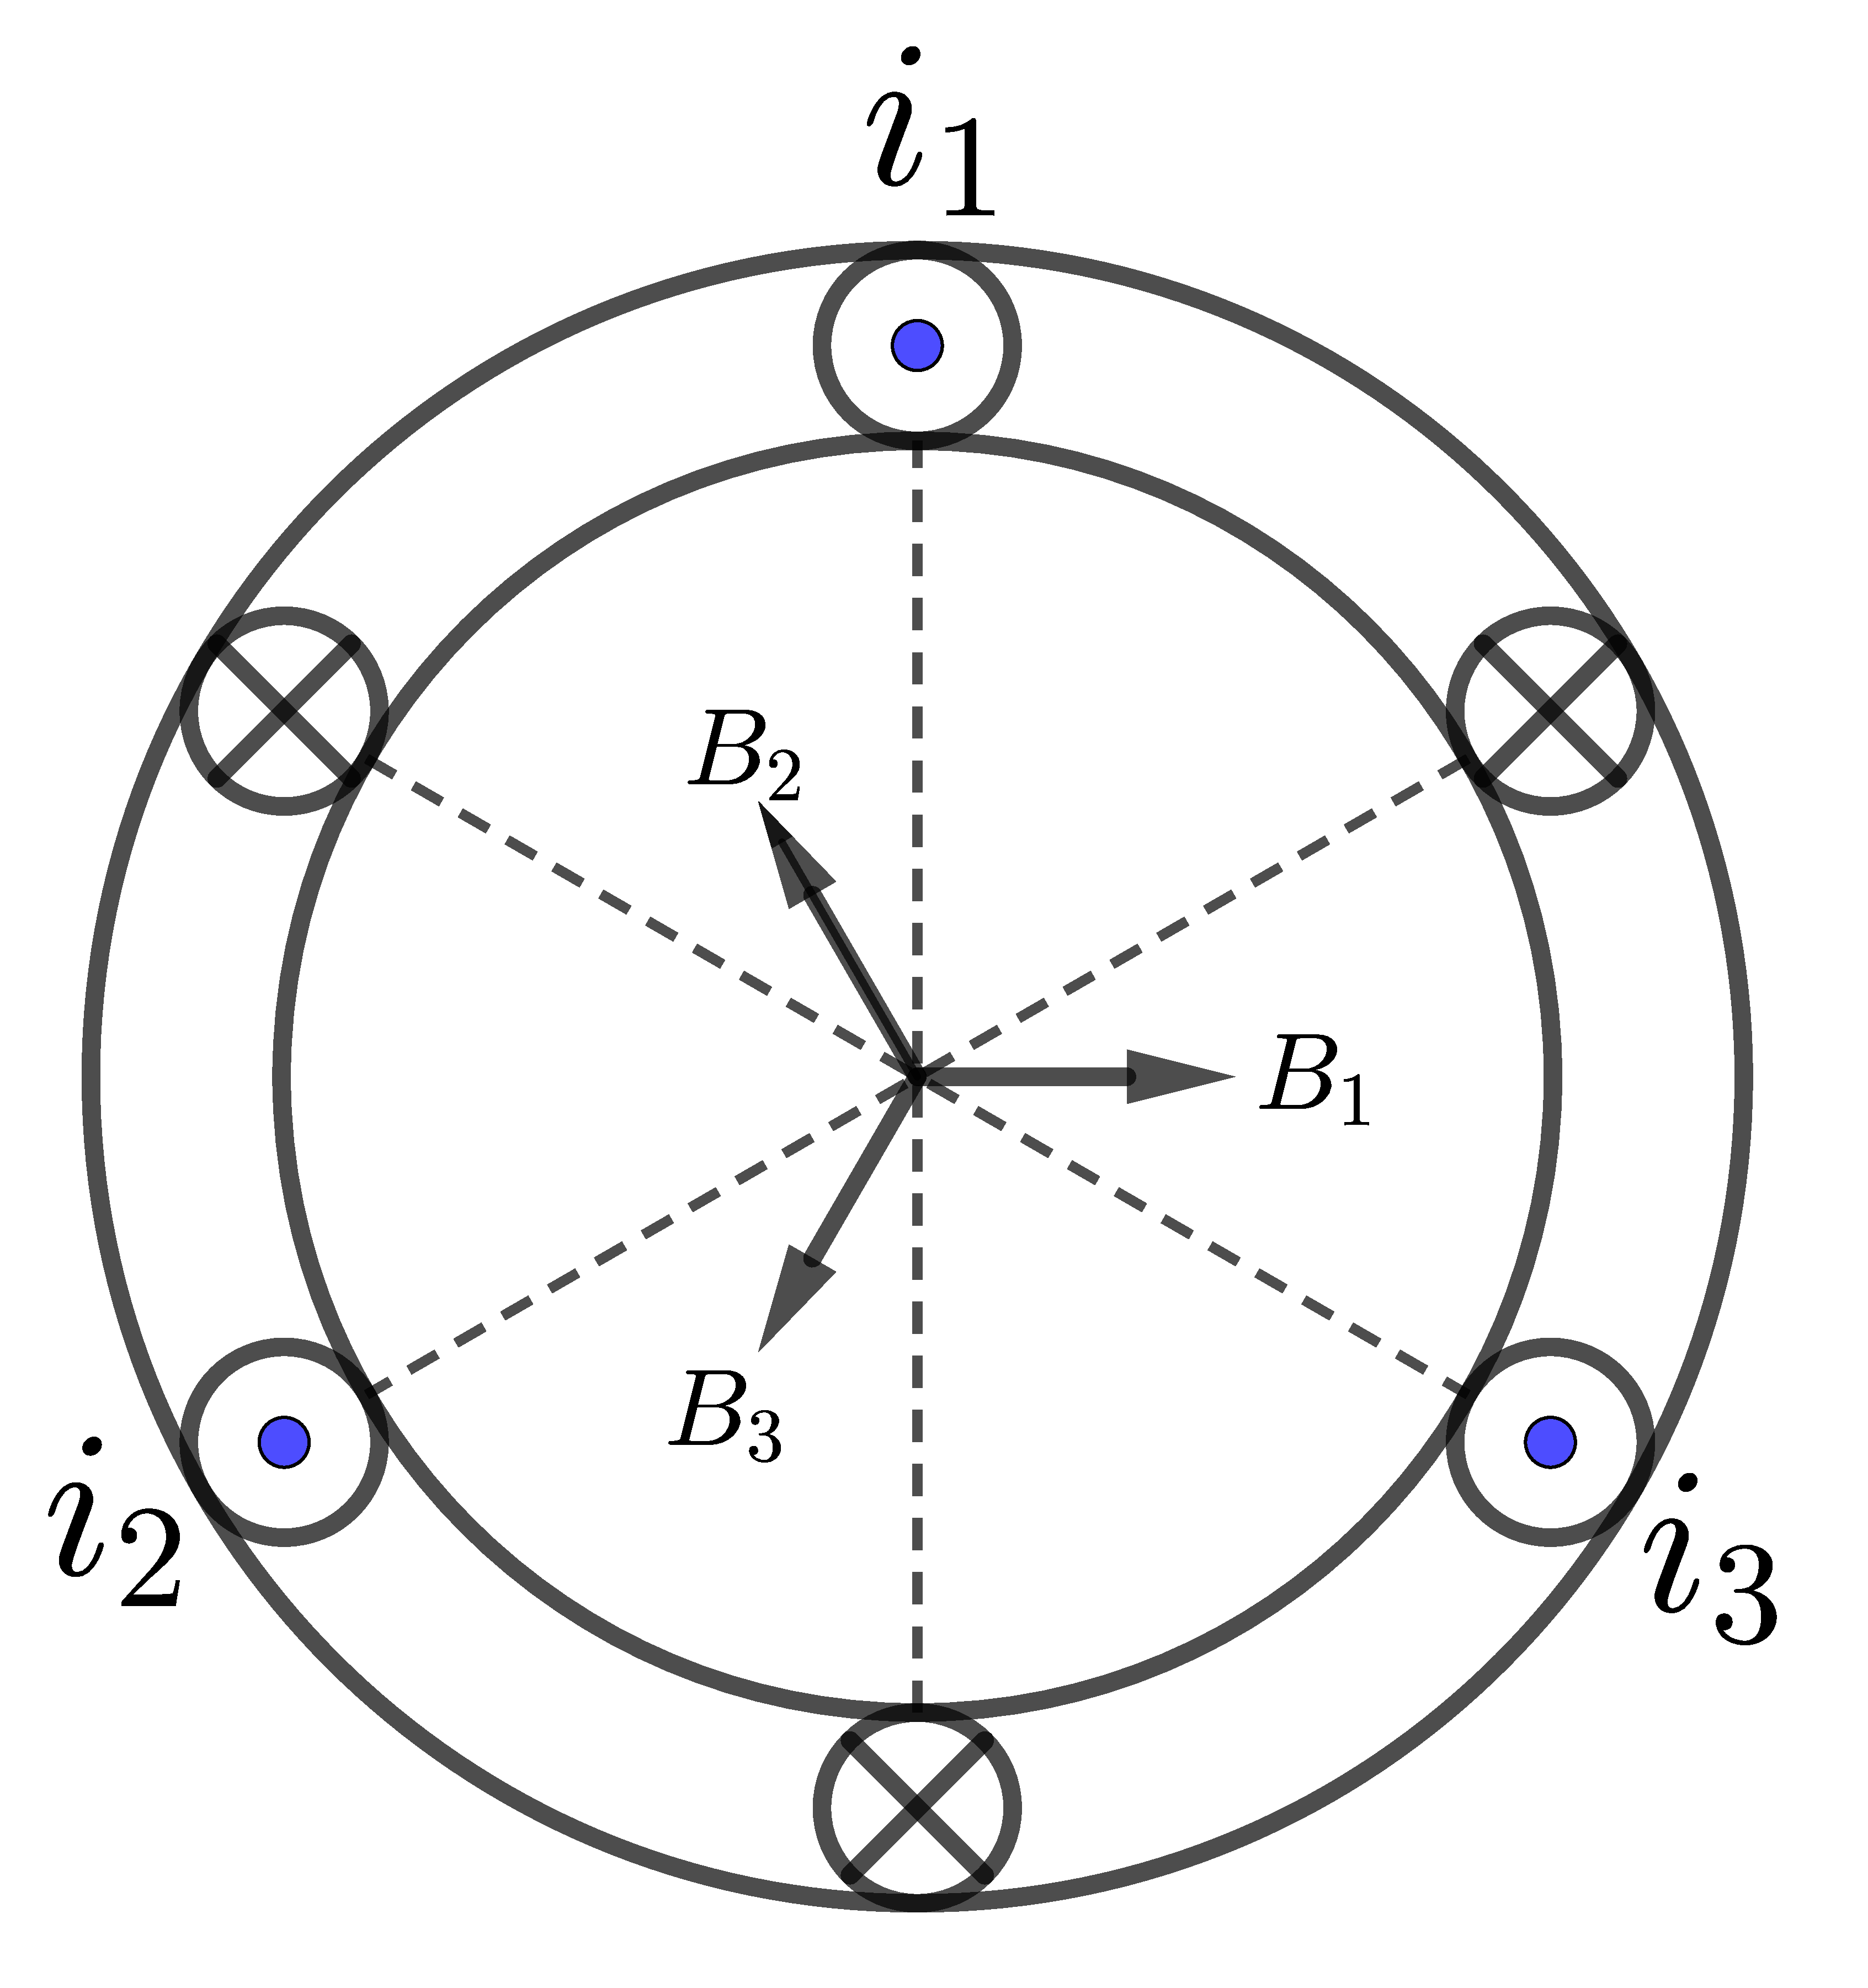
\includegraphics[width=0.35\textwidth]{电动机的基本构造.pdf}
	\caption{电动机的基本构造}
	\label{fig:电动机的基本构造}
\end{figure}
由电磁关系,我们不难知道它们形成的磁场应当为
\begin{equation*}
    \left\{ \begin{aligned}
        B_1&=B_m\sin \omega t\\
        B_2&=B_m\sin \left( \omega t+120\degree \right)\\
        B_3&=B_m\sin \left( \omega t-120\degree \right)\\
    \end{aligned} \right. 
\end{equation*}
同时,它们的方向也不同,见\href{https://www.geogebra.org/m/y9r93ads}{GGB上的动画}.

\Par 关于三相异步电动机的转速,当电动机只接有一个三相交流电的时候,最终形成的磁场只有一对南北极,由动画易知其频率与交流电频率相同
\begin{equation*}
    f_B=f_I
\end{equation*}
那么它的转速应当为
\begin{equation*}
    n=60f/\min 
\end{equation*}
而当它接了$p$个三相交流电,有$p$对南北极时,其转速为
\begin{equation*}
    n=60\frac{f}{p}
\end{equation*}
在我国$f=50\mathrm{Hz}$,因此

\begin{table}[htbp]
    \centering
    \begin{tblr}{row{odd} = {azure8}, 
        row{even} = {gray8},
        colspec={cccccc},
        }
        $p$ & 1 & 2 & 3 & 4 & 5\\
        $n\left( \mathrm{r}/\min \right) $ & 3000 & 1500 & 1000 & 750 & 600\\
    \end{tblr}
    \caption{$p$与$n$的关系}
\end{table}
\Par 同时,转子的转速应当小于磁场的转速,不然,转子无法切割磁感线,从而感应出电流受安培力形成转动.定义:\hl{转差率}$s$
\begin{equation}
    s\coloneqq \frac{n_0-n}{n_0}
\end{equation}
其中,$n$为转子转速,$n_0$为磁场转速,转差率$s$反映了转子转速$n$与磁场转速$n_0$的接近程度.
